\documentclass[11pt]{article}

\usepackage{sectsty}
\usepackage{graphicx}
\usepackage[left=0.5cm]{geometry}


\title{ Gestion de Asignaturas}
\author{ Quintero Angelica, Zambrano Pianina, Ramos Jurany, Ayoví Leah, Añapa Alex, Ulloa Alber }
\date{\today}

\begin{document}
\maketitle	
\section{Introduccion}

En respuesta a las demandas cada vez más complejas del
entorno educativo actual, presentamos un software de gestión de
asignaturas que simplifica y potencia la administración de
programas académicos. En un mundo educativo en constante
evolución, la gestión de asignaturas se ha vuelto esencial
para el éxito de las instituciones educativas y laexperiencia 
de aprendizaje de los estudiantes. Este software surge como
una solución integral para abordar el desafío crítico de la 
gestión de asignaturas, un tema de gran relevancia en la
educación contemporánea.


La necesidad de una plataforma que simplifique desde la
planificación curricular hasta la comunicación y
evaluación se vuelve cada vez más evidente. Este software se
destaca por su capacidad para centralizar la información
y la comunicación, permitiendo a educadores y estudiantes
interactuar de manera efectiva a través de una interfaz
intuitiva. Además, ofrece una amplia gama de herramientas
analíticas que permiten un seguimiento detallado del progreso
académico de los estudiantes y la identificación de áreas de
mejora. En este texto, exploraremos cómo este
software revoluciona la forma en que se gestionan las
asignaturas, presentando sus características clave y
discutiendo
cómo aborda los desafíos actuales en la educación. Esto
preparará el terreno para comprender en detalle las ventajas y
beneficios que ofrece en el ámbito educativo, allanando el
camino hacia una administración más efectiva y una
experiencia de aprendizaje enriquecida.
\section{Objetivo General}

El objetivo general de este estudio es analizar y demostrar
cómo el software de gestión de asignaturas presentado en
estetexto
revoluciona la administración de programas académicos en el
entorno educativo contemporáneo. Para lograr este propósito,
se llevará a
cabo una investigación exhaustiva que se centrará en las
características clave de esta plataforma, su capacidad para
simplificar laplanificación curricular, mejorar la
comunicación entre educadores y estudiantes, y proporcionar
herramientas analíticas avanzadas parael seguimiento del
progreso académico. Además, se explorarán los desafíos
actuales en la educación que este software aborda de manera
efectiva. El resultado final de esta investigación será
proporcionar una comprensión sólida y detallada de las
ventajas y beneficios que esta solución ofrece en el ámbito
educativo, con el objetivo de contribuir a una administración
más efectiva de los programas académicos y enriquecer la
experiencia de aprendizaje de los estudiantes.


\section{Objetivos Especificos}
\begin{enumerate}
\item Evaluar la capacidad del software de gestión de
asignaturas para simplificar la planificación
curricular:

*Analizar cómo el software facilita la creación de
programas académicos, horarios y asignación de recursos
educativos.

*Medir la eficiencia y efectividad del software en la
organización de planes de estudio, tareas
administrativas y gestión de recursos.

*Identificar las características específicas del
software que contribuyen a la simplificación de la
planificación curricular.

\item Examinar cómo el software mejora la comunicación entre educadores y estudiantes:

*Investigar cómo la plataforma facilita la interacción
entre docentes y alumnos, incluyendo la comunicación en
tiempo real y la colaboración en línea.

*Evaluar cómo el software contribuye a la transparencia
en la comunicación, permitiendo un seguimiento más 
cercano del progreso estudiantil.

*Identificar las herramientas de comunicación clave del
software y su impacto en la experiencia de aprendizaje.

\item Analizar las herramientas analíticas del software
para el seguimiento del progreso académico:

*Examinar las capacidades analíticas del software para
recopilar y procesar datos sobre el rendimiento
estudiantil.

*Evaluar la generación de informes y análisis de datos
proporcionados por el software.

*Determinar cómo estas herramientas ayudan a los
educadores a identificar áreas de mejora y tomar
decisiones informadas.

\item Explorar cómo el software aborda los desafíos
actuales en la educación:

*Identificar los desafíos comunes en la administración
académica y la experiencia de aprendizaje en el entorno
educativo actual.


*Analizar cómo el software aborda específicamente estos
desafíos, como la optimización de recursos, la
adaptación a entornos de
aprendizaje en línea y la gestión eficaz de datos.

*Comparar las soluciones propuestas por el software con
las prácticas tradicionales de gestión académica.

\item Presentar una comprensión detallada de las
ventajas y beneficios del software en el ámbito
educativo:

*Resumir de manera integral las ventajas clave del
software en términos de eficiencia administrativa,
mejora del rendimiento estudiantil y experiencia de
aprendizaje enriquecida.


*Destacar los beneficios específicos para educadores,
administradores escolares y estudiantes.


*Proporcionar ejemplos concretos y casos de uso que
ilustren cómo el software puede transformar la gestión
de asignaturas en
instituciones educativas. 
\end{enumerate}
\section{Modelo del sistema}
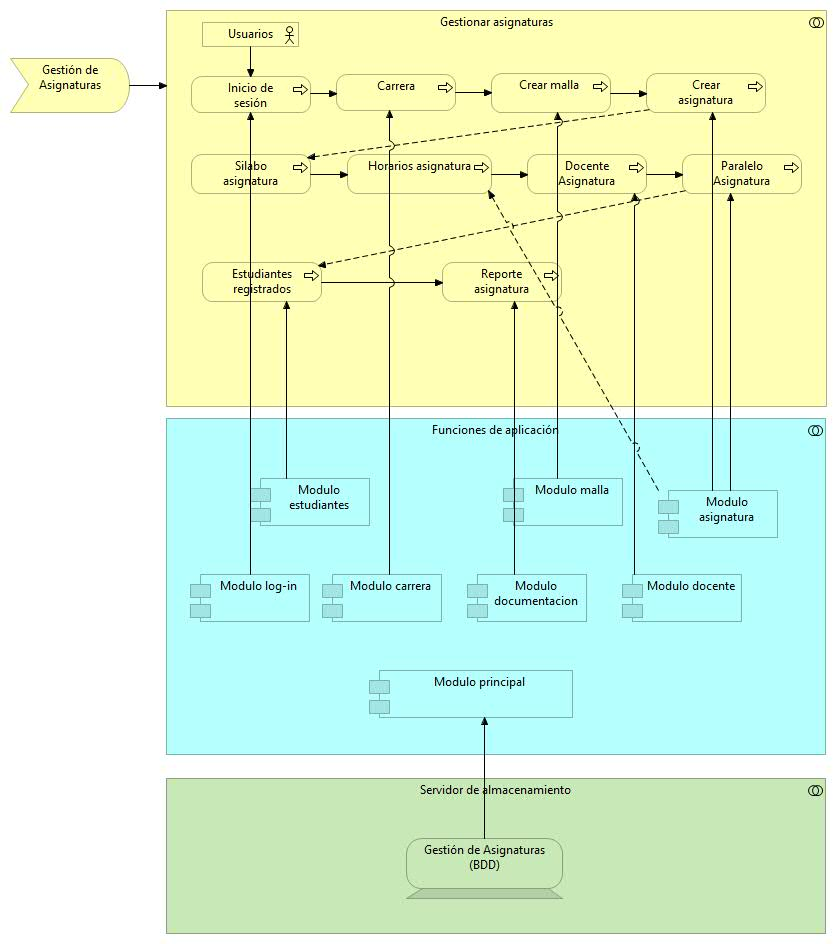
\includegraphics[scale=0.55]{ModelG.A.jpg}
\section{Prototipo}
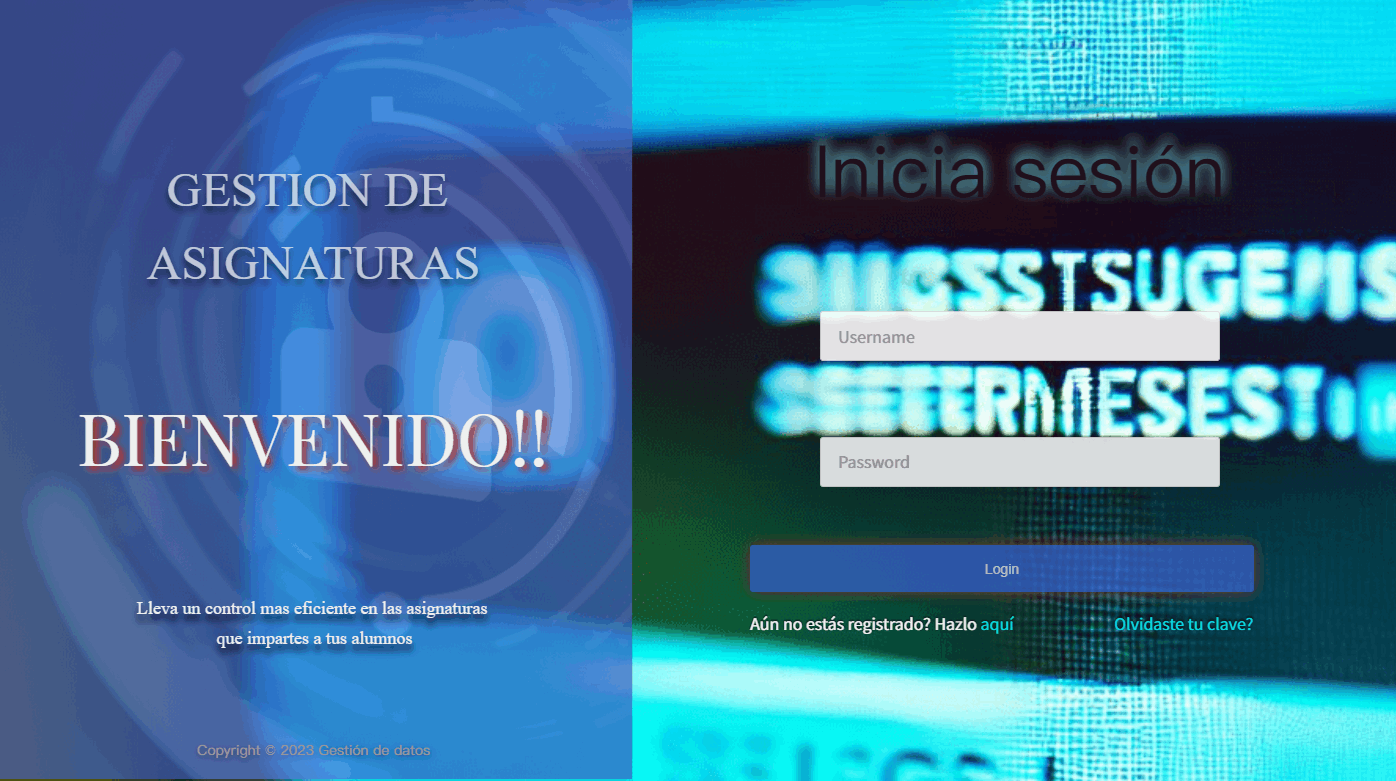
\includegraphics[scale=0.40]{0.png}
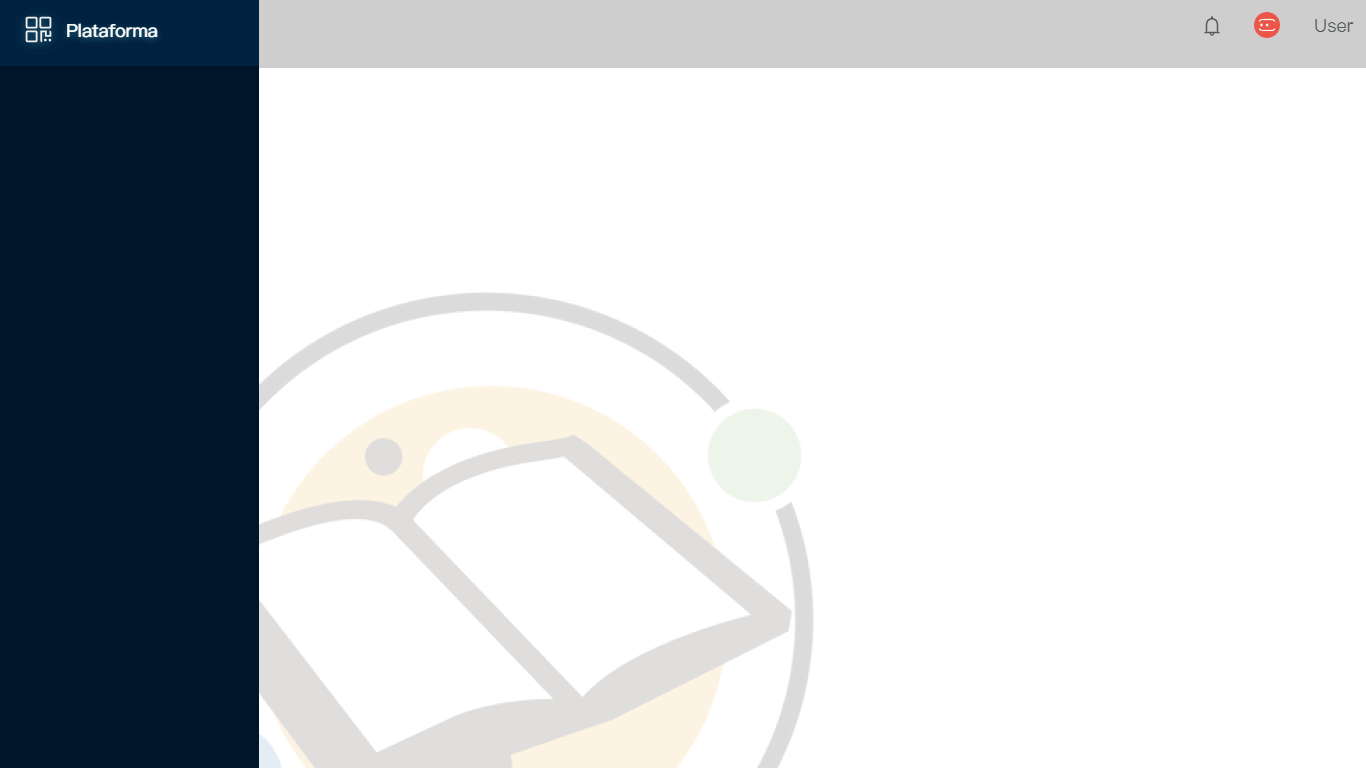
\includegraphics[scale=0.40]{1.png}
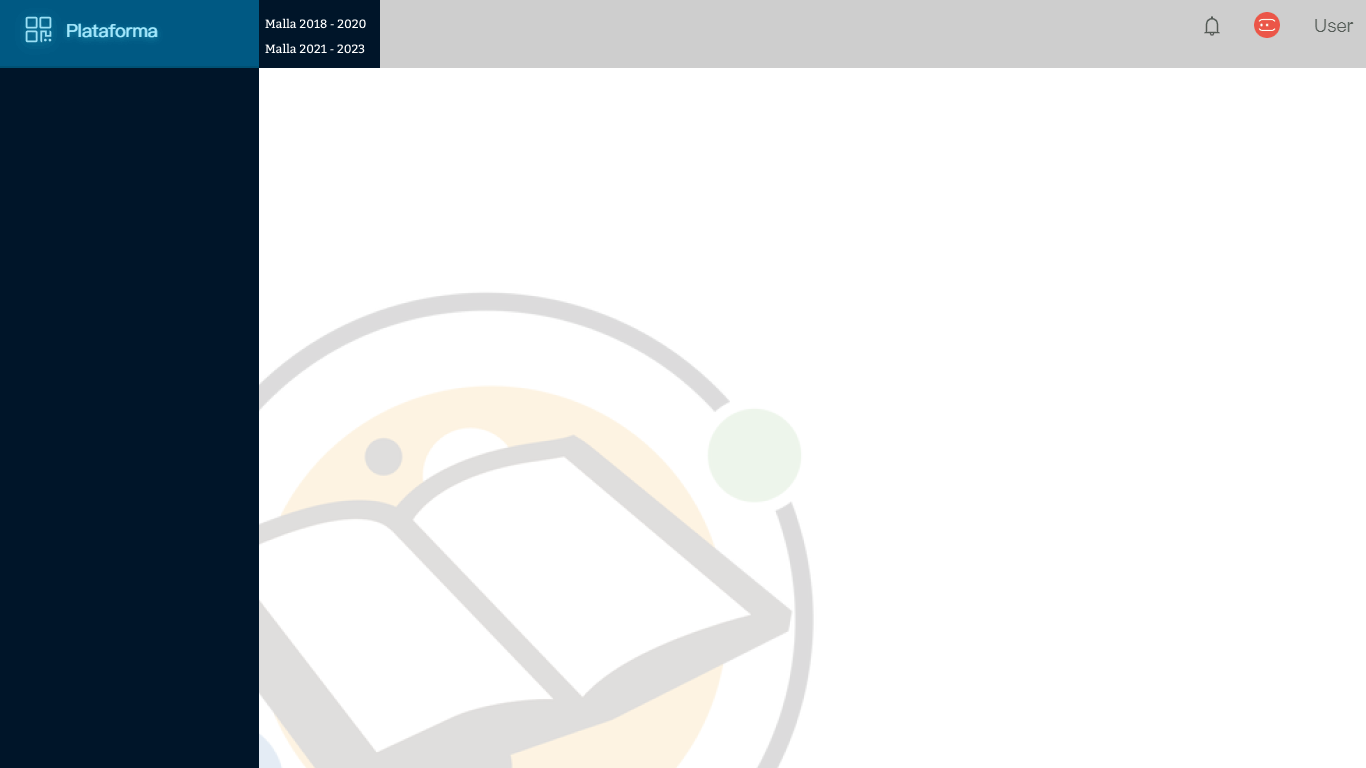
\includegraphics[scale=0.40]{2.png}
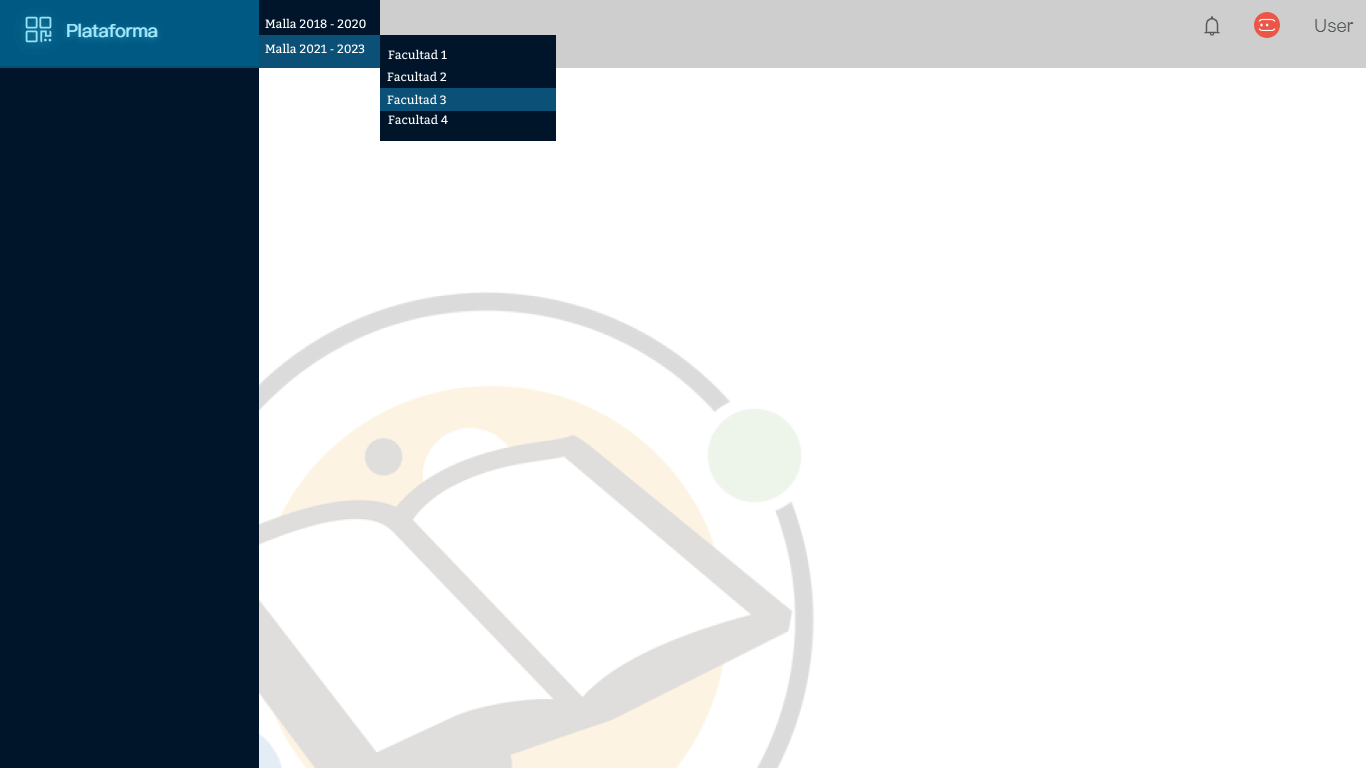
\includegraphics[scale=0.40]{3.png}
\end{document} 



